%%%%%%%%%%%%%%%%%%%%%%%%%%%%%%%%%%%%%%%%%%%%%%%%%%%%%%
\section{Introduction To The Standard Model}\label{secSM}



The Standard Model (SM) of particle physics is a quantum field theory (QFT) description of the strong, weak and electromagnetic forces of nature. The known particles of the SM are: 1 scalar Higgs boson, 4 gauge bosons, 6 types of quarks and 6 types of leptons. 

The quarks and leptons are fermions that constitute matter and so obey Fermi-Dirac statistics due to their half-integer spin. In contrast, the bosons have integer spin and obey Bose-Einstein statistics. Gauge bosons mediate the 3 fundamental forces and the Higg's boson is responsible for the electro-weak symmetry breaking which gives mass to the other particles~\cite{Griffiths:111880}. 

% rivello: Error below on \cite{fig:SM}
The fermions are arranged into 3 generations, arranged in columns from left to right on ~\ref{fig:SM}

\begin{figure}[htb]
\centering
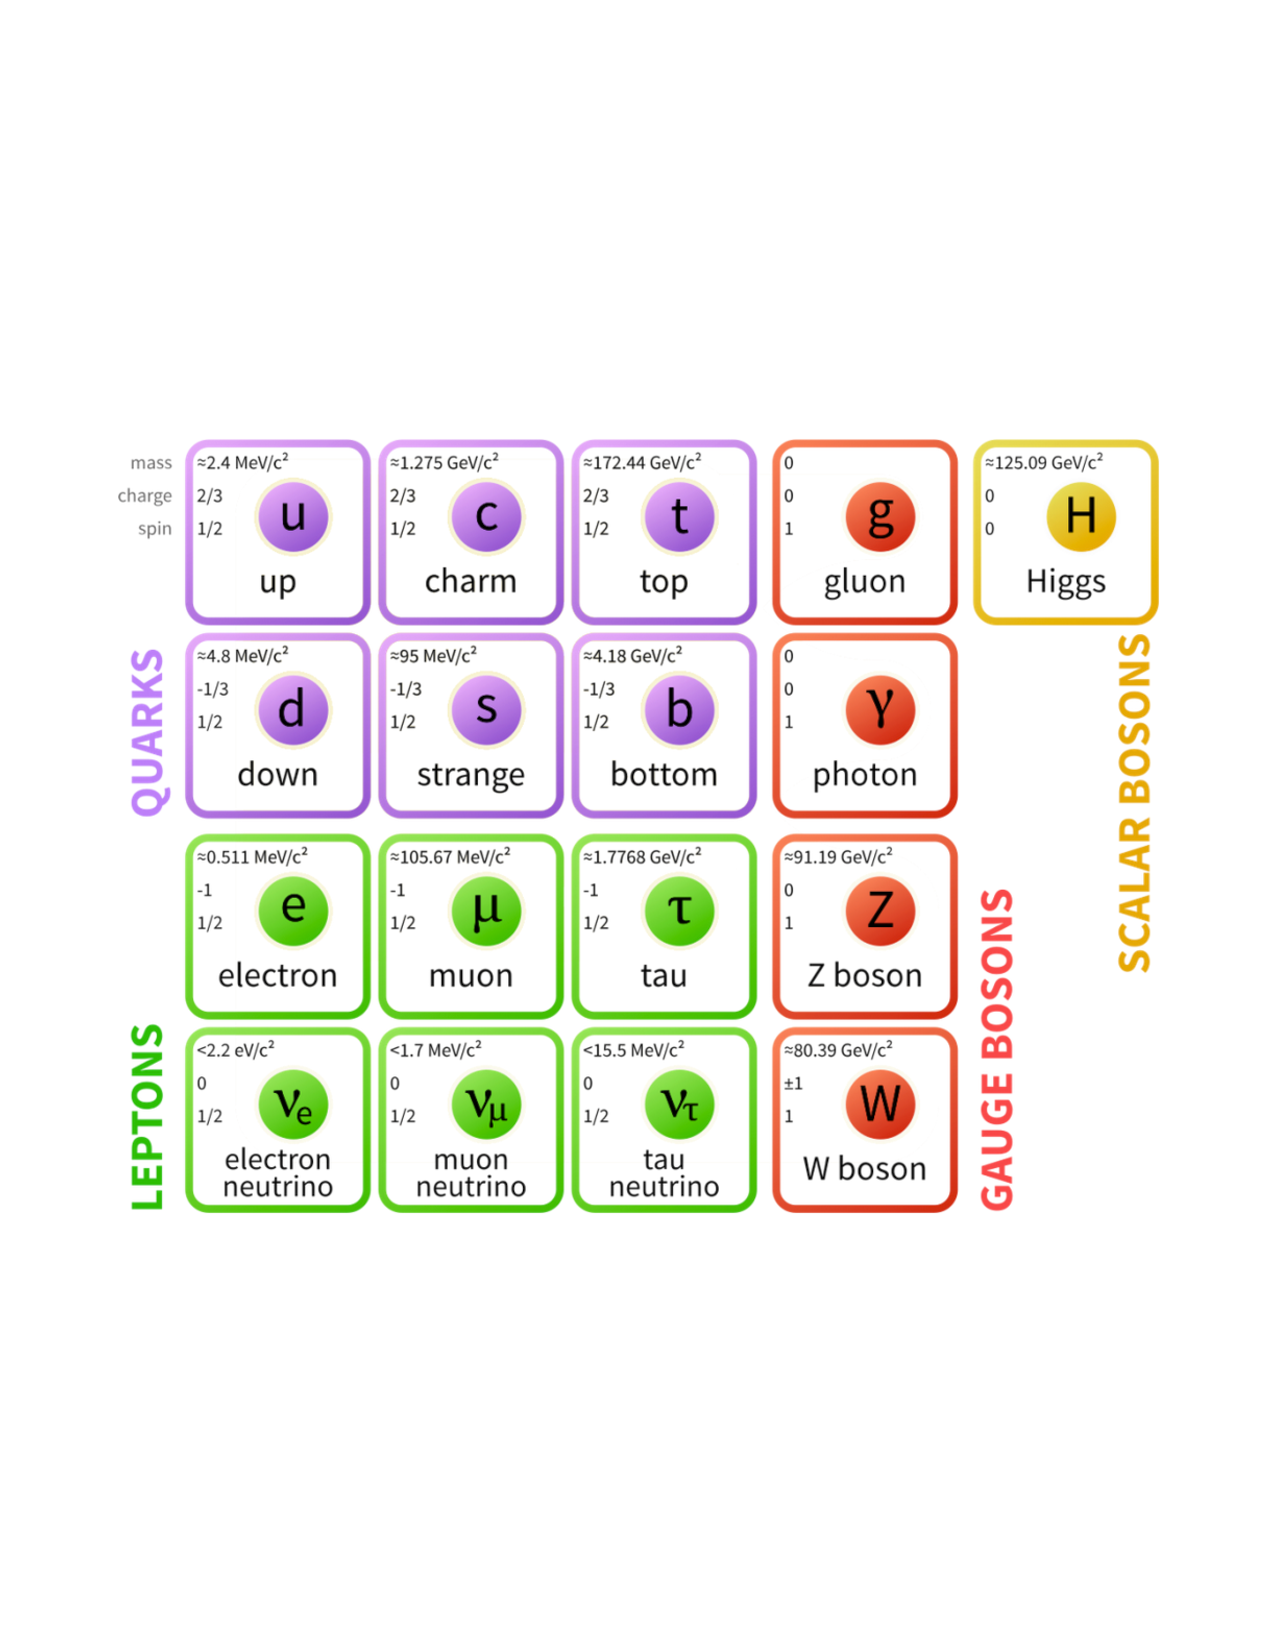
\includegraphics[width=.60\textwidth]{smdiagram.pdf}
\caption{Fundamental particles of the Standard Model~\cite{modellinginvisible}.}
\label{fig:SM}
\end{figure}




The SM is humanity's most rigorous theory of our universe, providing predictions of observables that have since been measured, in the case of Quantum Electrodynamics, QED, to the highest precision of any scientific theory. Despite the impressive predictions, the gravitational force and more subtle phenomena, such as flavor oscillation of neutrinos ~\cite{Ashie:2005ik}, indicate the existence of physics beyond the standard model, BSM.

Various attempts have been made to unify the fundamental forces under one theory, thus far the electromagnetic and weak interactions have been united by electro-weak theory. 

The Standard Electroweak Model can be described $SU(2) x U(1)$ mathematically.
% rivello: remember to fix paragraph below.
The  $SU(2) x U(1)$ gauge group is a unification of the special unitary symmetry group $SU(2)$ describing 3 mixed massive vector bosons, ($W_{-}$ $W_{+}$ $Z_0$), as carriers of the weak nuclear force, and the unitary gauge group $U(1)$ , describing the massless chargeless photon, of the electromagnetic interaction.

The standard model of the strong interaction is known as Quantum Chromodynamics, QCD, a non-Abelian gauge theory described by the special unitary group $(SU(3)_c)$, where the flavours of quark are the physical manifestation of the symmetry group. This force is mediated by the 8 massless gluons that carry color charge, making QCD more complicated mathematically than QED.

The SM also contains a Higgs boson, an excitation of a scalar Higg's field, which gives rise to spontaneous symmetry breaking of the electroweak theory, providing the particles with mass, but that won't be discussed herein. 

The quarks and leptons are arranged in generations according to their relative masses, as shown in Figure \ref{fig:SM}. The table also shows the spins of the particles, the leptons and quarks have half-integer spin, fermions, that obey the fermi exclusion principle. Conversely, the bosons have half integer spin and therefore obey bose-einstein statistics. Through the SM we interpret the observed hadronic particles, mesons ( baryons ), as 2 quark (3 quark) bound states. The existence of spin $\frac{3}{2}$ baryons, which are symmetric bound states in space, spin and flavour, and the need to obey Fermi-Dirac statistics, by maintaining total assymmetry of the wave function, implies there is another degree of freedom, called color, so that each quark is either red, green or blue. Granted only color singlet states exist. Furthermore there exists a property of asymptotic freedom where the QCD coupling between quarks and gluons increases as they asymptotically approach one another. There exist a wealth of experimental data to support the concept of asymptotic freedom. Asymptotic freedom is a useful property as it allows for perturbative calculations of QCD observables, such as the jet mass, this is discussed in ~\ref{sec:jetmass}. The running of the QCD (strong) coupling constant as measured by CMS experiment can be seen in ~\ref{fig:alphas}


\begin{figure}[htb]
\centering
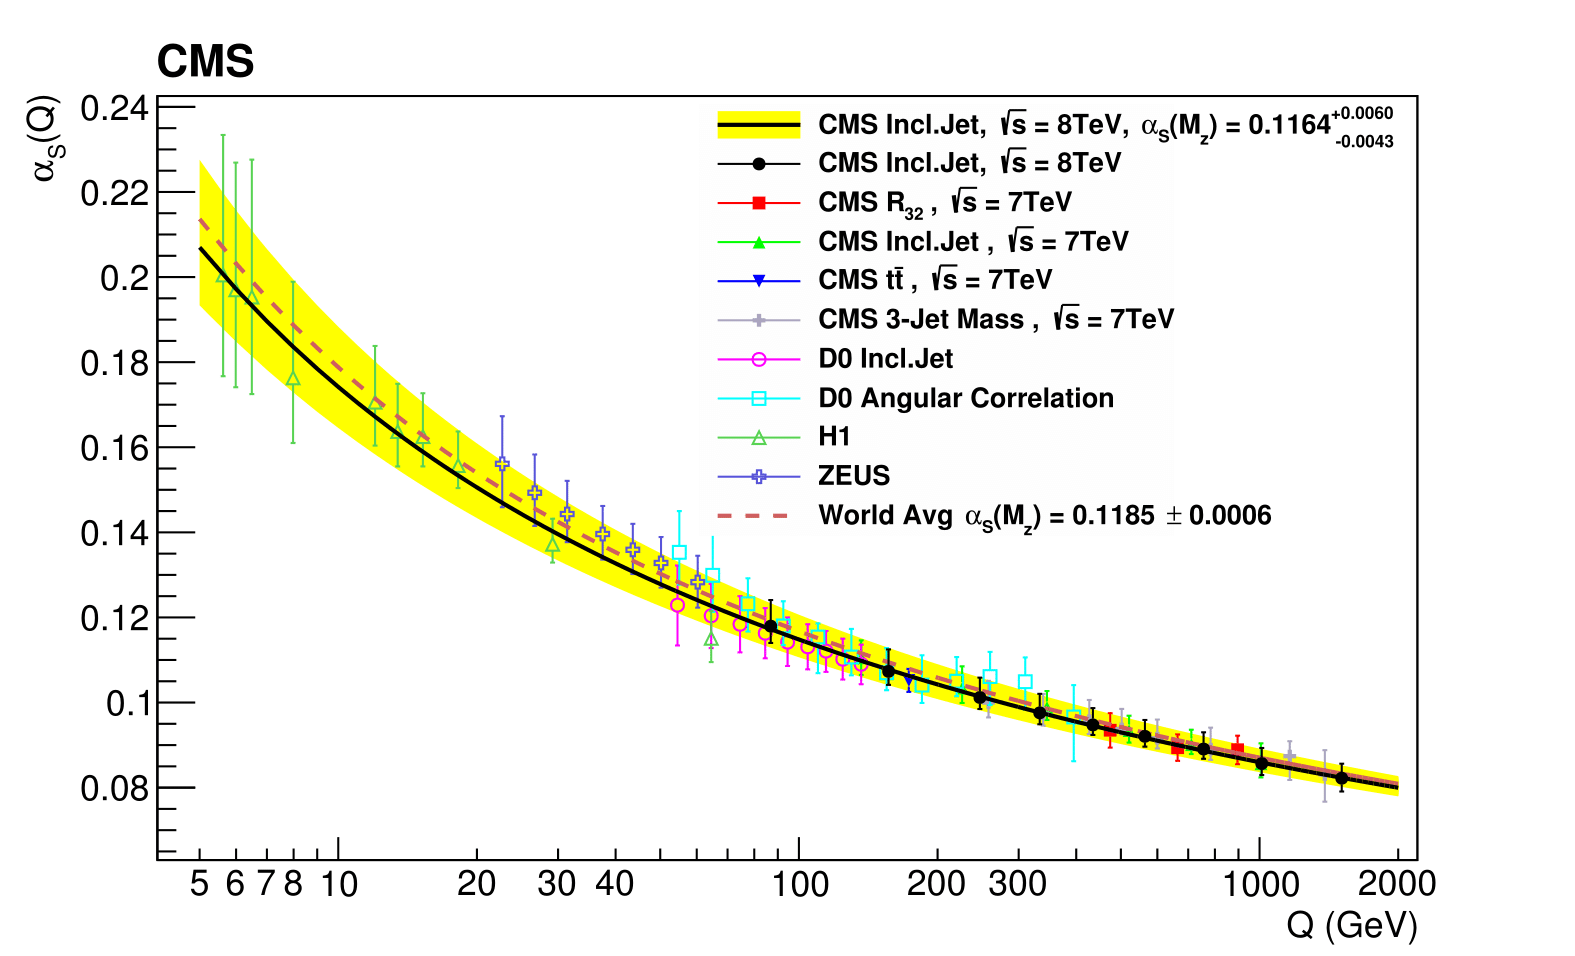
\includegraphics[width=.70\textwidth]{visuals/strong-coupling-cms2.png}
\caption{The running of the strong coupling constant as compiled by CMS including measurements from CMS and HERA among others~\cite{CMS:2014mna}.}
\label{fig:alphas}
\end{figure}


%image CMS:2014mna
% visuals/strong-coupling-cms






%another DY thesis  http://inspirehep.net/record/1345977/files/DoolingSamantha_Dissertation.pdf


% Symmetris imply conserved quantities, Neuther's Theorem


Nuclei in ordinary matter are composed solely of $1^{st}$ generation particles, up and down quarks, bound by gluons. Neutral atoms contain an equal number of protons (composed of 2 up quarks and a down quark) and electrons, $1^{st}$ generation leptons. The main distinction between leptons and quarks, both fermions (particles of $\frac{1}{2}$ integer spin), being that leptons do not experience the color interaction $(SU(3)_c)$ like their quark friends. In each generation there is a quark with charge $Q = + \frac{2}{3}$ (up, charm, top) and another of charge $Q = - \frac{1}{3}$ (down, strange, bottom).





\subsection{Quantum Chromodynamics}\label{secQCD}


QCD is a quantum field theory that describes the color force, experienced by quarks and mediated by gluons. The quarks each posess a color charge ; red, green or blue (anti-red, anti-green or anti-blue). In contrast the gluons are "bicolored", each carrying one unit of negative and one of positive charge.~\cite{Griffiths:111880}. As previously metioned, QCD a non-Abelian gauge theory described by the special unitary group $(SU(3)_c$ (color charge) and has a Lagrangian that can be written as follows:\newline


\begin{equation}
\mathcal{L}=-\frac{1}{4} F_{\mu \nu}^{A} F_{A}^{\mu \nu}+\sum_{\text {flavours }} \overline{\psi}_{a}\left(i \gamma_{\mu} D^{\mu}-m\right)_{a b} \psi_{b}
\end{equation}


The sum is over each of the generators of the $(SU(3)_c$ gauge group, and the quark field fermion multiplets, $\psi$, belong to its irreducible representation.~\cite{Crewther:1995wq}

The gluon fields $A_{\nu}^a$ of spin 1 have a field strength tensor, $F_{\mu \nu}^{A}$ , given below:\newline 

\begin{equation}
F_{\mu \nu}^{A}=\partial_{\mu} A_{\nu}^{A}-\partial_{\nu} A_{\mu}^{A}+g_{s} f^{A B C} A_{\mu}^{B} A_{\nu}^{C}
\end{equation}


The structure functions are denoted as $f^{A B C}$ and their indicies run over all of the gluon color degrees of freedom. It is noteable to mention that the third term in the above equation is what gives rise to asymptotic freedom through the gluon quartic and triple self-interactions it induces ~\cite{Crewther:1995wq}.

The covariant derivative is defined as :\newline

\begin{equation}
\left(D_{\mu}\right)_{a b}=\partial_{\mu} \delta_{a b}-i g_{s} A_{\mu}^{A} t_{a b}^{A}
\end{equation}

Where the $t_{a}$ are the matrices of the fundamental representation of $(SU(3)$.

Lastly, for completeness, I mention the final gauge invariant term of the QCD Lagrangian below, where $\theta_{QCD}$ is a free parameter of QCD known as the vacuum angle parameter.

\begin{equation}
\mathcal{L}_{\theta}=\theta_{\mathrm{QCD}} \frac{\alpha_{s}^{2}}{64 \pi^{2}} \epsilon^{\mu \nu \rho \sigma} F_{\mu \nu}^{a} F_{\rho \sigma}^{a}
\end{equation}


QCD is discussed from a phenomenological perspective in ~\ref{sec:quarkandgluonjets}. 








%%%%%%%%%%%% NEW  CHAPTER %%%%%%%%%%%%%%%%%%%%





